
% !TeX root = Bericht_main.tex



\subsection{Aufgabe 21}

Wir wollen im Folgenden auf die in Aufgabe 21 beschriebenen Probleme eingehen:
Wir betrachten zu einem gegebenen Vektorfeld $q$ mit $ \dive q = 0$ die lineare Transportgleichung als Rand-Anfangswertaufgabe (RAWP),
\begin{align*}
 	\partial_t \rho + \dive (\rho q) &= 0  &&\text{auf }\Omega \times [0,T] \\
 	\rho(0) &= \rho_0   &&\text{auf } \Omega \\
 	\rho &= \rho_{in}  &&\text{auf } \Gammain = \{ x \in \partial \Omega: q \cdot n < 0 \} \times [0,T]
\end{align*}
welches mit Hilfe von Finite Volumen- bzw. discontinuous Galerkin Verfahren gelöst werden soll. Dabei betrachten wir die folgenden zwei Probleme:

\subsubsection{Problem A (Riemann-Problem)}
Wir setzen: 
\begin{align*}
	\rho_{in} &= 0 \\
	\rho_0 &= 1 \qquad y \in (7,9), x \in (0,10)
\end{align*}
\begin{figure}[H]
	\centering
	\captionabove{Anfangsbedingungen}
	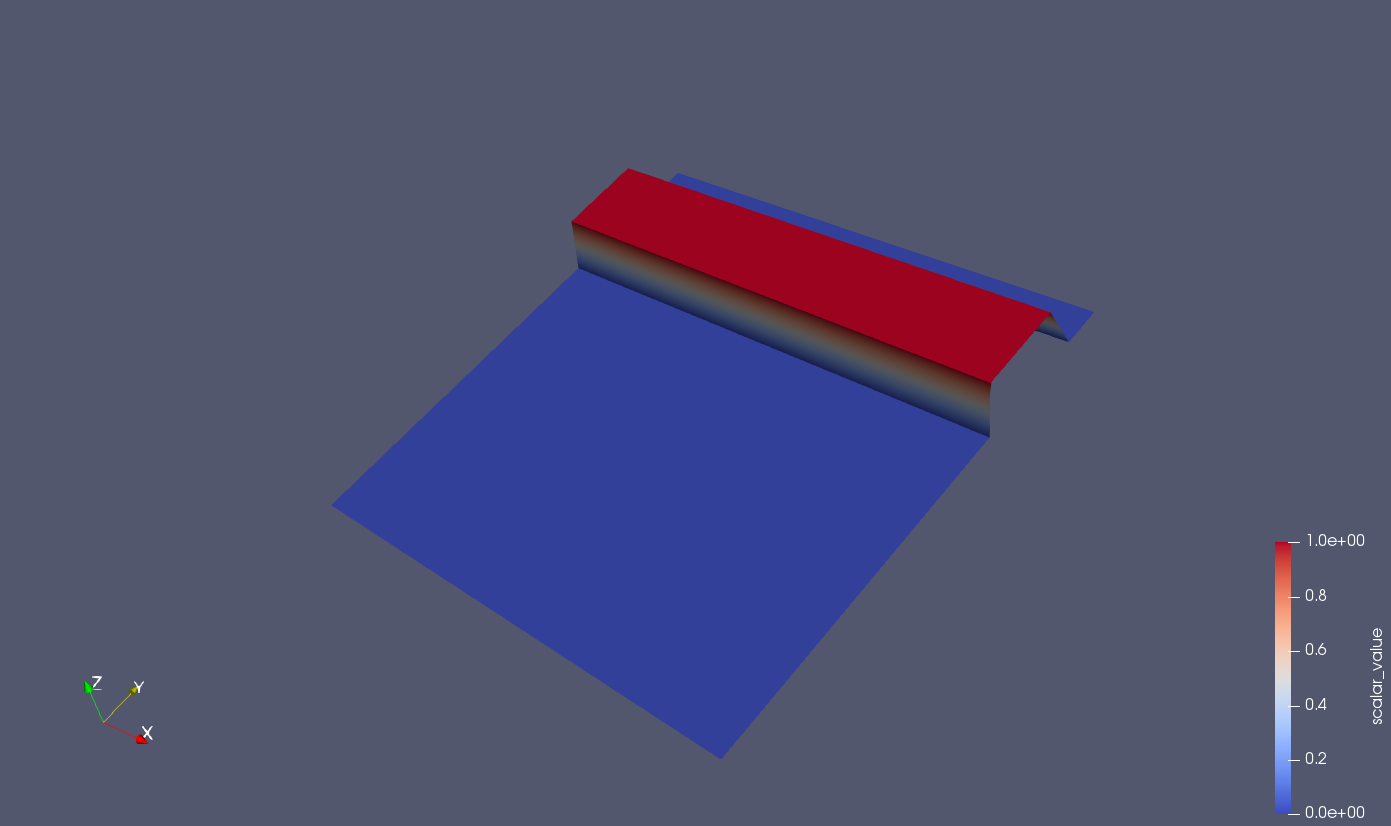
\includegraphics[width=\textwidth]{../TransportRk-2_dt003125lvl6/animation1.png}
\end{figure}
\begin{figure}[H]
	\centering
	\captionabove{Lösung des Riemann-Problems mit FV-Verfahren und der impliziten MPR als Zeitintegrator}
	\subfigure[t=0,125]{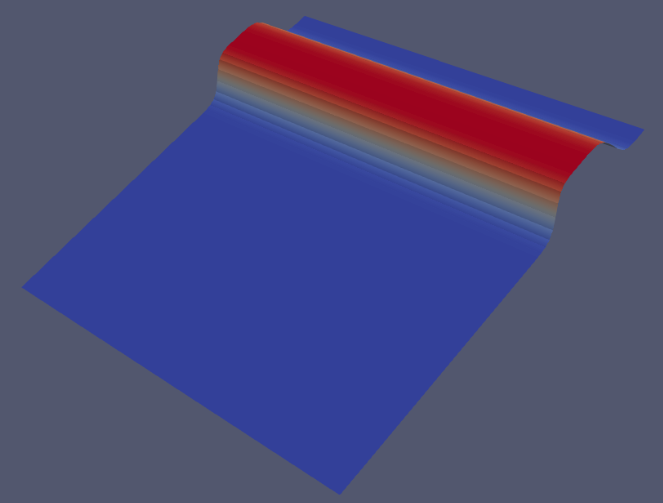
\includegraphics[width=0.47\textwidth]{../Aufgabe21/rieanm1.png}}
	\subfigure[t=1,875]{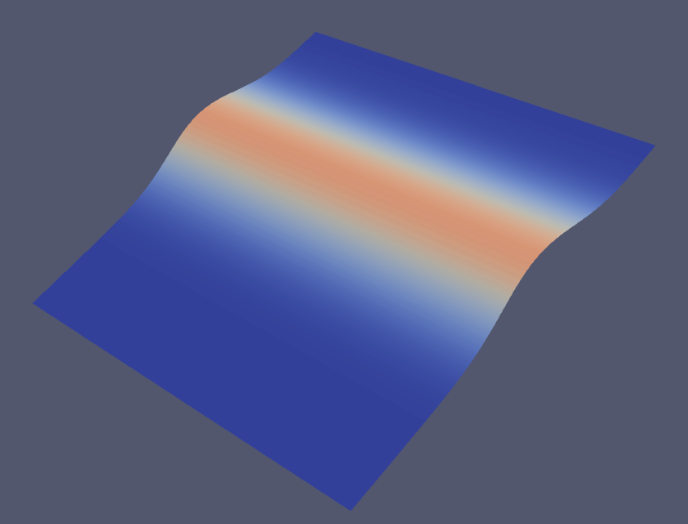
\includegraphics[width=0.47\textwidth]{../Aufgabe21/rieanm2.png}}
	\subfigure[t=6,5]{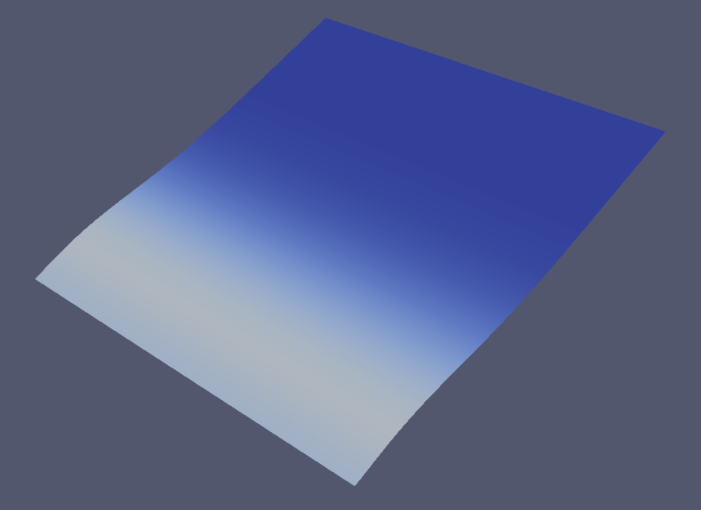
\includegraphics[width=0.48\textwidth]{../Aufgabe21/rieanm3.png}}
\end{figure}
\begin{remark}(Analytische Betrachtung) \newline
Sei $\Omega = \R ^D$ , $q_0 \in \R ^D$ , $n_0 \in \R ^D$ und 
	\begin{align*}
		\rho_0 (x) &= 
			\left\{              
				\begin{array}{r l}
					\rho_- , \qquad x \in \Omega_- &\coloneqq \{x \in \Omega : x \cdot n_0 < 0 \} \\
					\rho_+ , \qquad x \in \Omega_+ &\coloneqq \{x \in \Omega : x \cdot n_0 > 0 \}
				\end{array}
			\right.  \\
			\Rightarrow \rho (x,t) &= 
				\left\{              
					\begin{array}{r l}
						\rho_- , \qquad x \in Q_- &\coloneqq \{(x,t) \in \Omega \times [0,T] : (x - tq_0) \cdot n_0 < 0 \} \\
						\rho_+ , \qquad x \in Q_+ &\coloneqq \{(x,t) \in \Omega \times [0,T] : (x - tq_0) \cdot n_0 > 0 \} 
					\end{array}
				\right. 
	\end{align*}
	ist schwache Lösung, denn für eine beliebige Testfunktion $\phi \in C_0^{\infty} ([-1,T] \times \R^D)$ gilt:
	\begin{align*}
		&\int_{\Omega} \rho_0 \phi (0) dx + \int_{Q_- \cap Q_+ } 
				\begin{pmatrix}
       				\rho \\
       				\rho q_0
     			\end{pmatrix}
     		\cdot
     			\begin{pmatrix}
       				\partial_t \\
       				\nabla q_0
     			\end{pmatrix}
     		\phi \; dxdt  \\
     	= &\int_{ \partial Q_- \cap \partial Q_+ } \rho_- \phi
     		\begin{pmatrix}
       				1 \\
       				q_0
     			\end{pmatrix}
     		\cdot
     			\begin{pmatrix}
       				-q_0 \cdot n_0 \\
       				n_0
     			\end{pmatrix} 
     		\; da dt
     	+ \int_{ \partial Q_- \cap \partial Q_+ } \rho_+ \phi
     		\begin{pmatrix}
       				1 \\
       				q_0
     			\end{pmatrix}
     		\cdot
     			\begin{pmatrix}
       				-q_0 \cdot n_0 \\
       				n_0
     			\end{pmatrix} 
     		\; da dt	
	\end{align*}
	Wir können also tatsächlich analytisch eine Lösung des Problems berechnen und wollen nun untersuchen, wie sich das Finite Volumen Verfahren mit zwei verschiedenen Lösungsverfahren zur Zeitintegration verhält. 
	\end{remark} 
	Genauer betrachten wir hierbei zunächst das explizite Runge-Kutta-Verfahren 4. Ordnung und wenden uns danach der impliziten Mittelpunktsregel zu (diese hat Ordnung 2). Besonders wollen wir dabei auf die sogenannte CFL-Bedingung, eine Stabilitätsbedingung für explizite Verfahren,  $\mathcal{O}(\frac{\Delta t}{h})$ bzw. $\Delta t < Ch$ eingehen. Dabei ist das $\Delta t$ die Schrittweite der Zeitdiskretisierung und $h = \frac{10}{2^{level} }$ die Schrittweite der Ortsdirskretisierung. 
	Dazu vergleichen wir die transportierte Energie für die Finite Volumen Raumdiskretisierung auf unterschiedlichen Levels mit den beiden genannten Zeitintegratoren.

\begin{figure}[H]
	\centering
	\captionabove{Energiewerte für das explizite Runge-Kutta-Verfahren 4. Ordnung}
	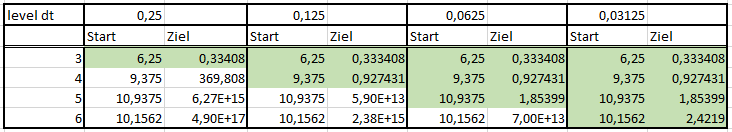
\includegraphics[width=\textwidth]{../Aufgabe21/tabellefarbig.png}
\end{figure}
\begin{remark}
	Bei allen nicht grün gefärbten Zielwerten bis auf Level 4 bei dt 0,25 handelt es sich um den Wert der Energie zum Zeitpunkt $\tilde{t}<T$,  bei dem das Programm aufgrund der auftretenden Divergenz stoppt.
\end{remark}
Anhand obiger Tabelle lässt sich die bereits genannte CFL-Bedingung für die Stabilität des Zeitintegrators sehr leicht nachvollziehen. \newline
Für die Zeitschrittweite $\Delta t = 0,25$ liefert nur Level 3 ein vernünftiges Ergebnis. Für Level 4 ist die Energie zum Zielzeitpunkt T bereits jenseits der Größenordnung der zu Beginn vorhandenen Energie, bei Level 5 und 6 sieht man sogar noch besser, dass die Lösung divergiert. Diese Ergebnisse lassen sich mit der CFL-Bedingung erklären: \newline
Während wir bei Level 3 noch 
\begin{align*}
	\Delta t = 0,25 < C \cdot 1,25  = Ch
\end{align*} 
erhalten, gilt $ \Delta t < Ch$ für die Levels 4 bis 6 allerdings nicht mehr.
Halbieren wir nun aber die Zeitschrittweite $\Delta t$, so konvergiert der Zeitintegrator auch für Level 4, denn
\begin{align*}
	\Delta t =0,125 =  \frac{1}{2} \cdot 0,25 < C \cdot  \frac{1}{2} \cdot 1,25  =C \cdot 0,625 = Ch
\end{align*}
Wie man also auch anhand der Tabelle schön sieht erhalten wir für jede Halbierung der Zeitschrittweite ein weiteres Level, auf welchem das explizite RK-Verfahren 4.Ordnung konvergiert. 

\begin{figure}[H]
	\centering
	\captionabove{Energiewerte für die implizite Mittelpunktsregel}
	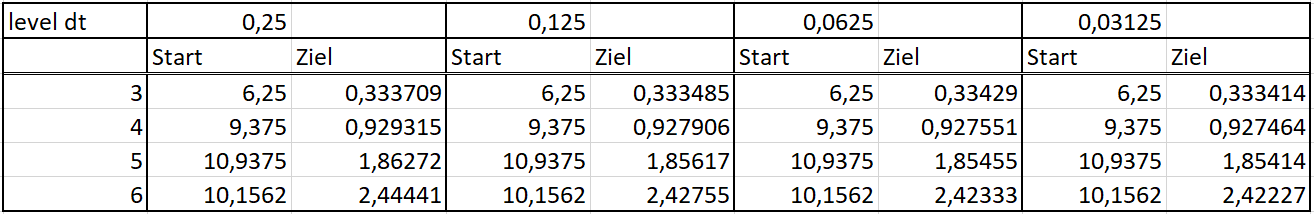
\includegraphics[width=\textwidth]{../Aufgabe21/rkorder-2RiemannEnergieTabelle.png}

\end{figure}
Im Gegensatz dazu sieht man bei Verwendung der impliziten Mittelpunktsregel, dass diese ohne CFL-Bedingung stabil ist und somit keine Divergenzen auftreten. Grund dafür ist, dass die implizite Mittelpunktsregel sogar A-stabil ist.
Allerdings sind dafür die resultierenden Energiewerte für den Zeitpunkt T nicht mehr so schön konstant beim Vergleich verschiedener Zeitschrittweiten wie zuvor bei den (konvergenten) Werten vom expliziten RK-Verfahren.
Während zuvor die Energiewerte zum Zeitpunkt T (im Falle der Konvergenz) stets übereinstimmten, unabhängig davon mit welcher Zeitschrittweite gerechnet wurde, erhalten wir nun schwach schwankende Ergebnisse. Dies liegt an der schlechteren Ordnung des verwendeten Zeitintegrators (implizite Mittelpunktsregel), vgl. Übungsblatt 9 Aufgabe 31.
Betrachtet man zudem noch den zeitlichen Verlauf der Masse und Energie, erhält man Ansätze dafür, wie die Fehler zur exakten Lösung zu den unterschiedlichen Zeitpunkten entstehen.
\begin{figure}[H]
	\centering
	\captionabove{Zeitverlauf von Energie/Masse beim Lösen des Riemannproblems (Level 6, dt 0,03125, Rk4)}
    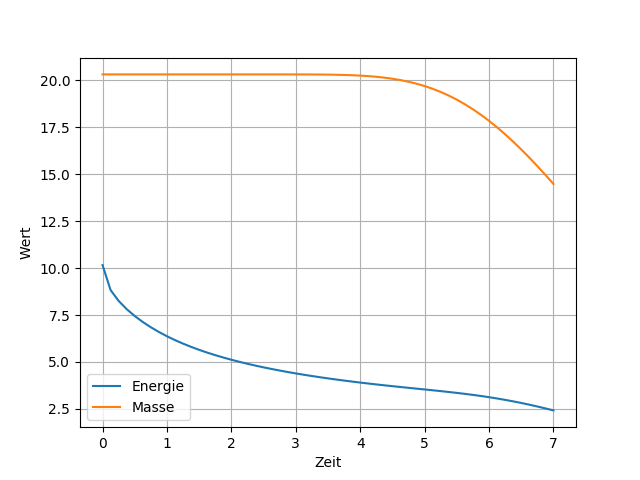
\includegraphics[width=0.8\textwidth]{../Aufgabe21/zeitverlauf.png}
\end{figure}
Wir erklären zunächst das Verhalten der Masse und gehen danach kurz auf die Energie ein:

\begin{figure}[H]
	\centering
	\captionabove{Masse, Outflowrate und Inflowrate über die Zeit geplottet bei rkorder = -2, deg = 0, lvl = 6}
	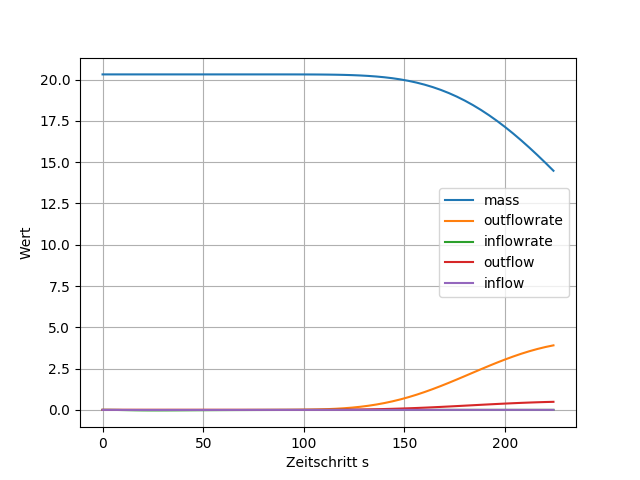
\includegraphics[width=0.8\textwidth]{../Aufgabe21/plotraten2.png}
\end{figure}
\remark Wir werden Outflow und Inflow gleich noch erläutern.
\newline
Wir erhalten dabei als Werte:
\begin{itemize}
	\item Masse bei $ t = 0 $: 20.3125
	\item Masse bei $ t = 7 $: 14.4885
\end{itemize}



Wir versuchen nun den Masseverlust durch die entstehenden Ein- und Ausflüsse zu erklären. Dazu berechnen wir aus Ein- und Ausflussrate jeweils den Gesamtein- bzw. ausfluss.
Dazu approximieren wir das Integral über die Zeit der Raten $r_{in}(t)$ und $r_{out}(t)$ wie folgt:
\begin{align*}
	\int_0^7 r_{in}(t) dt &\approx \sum\limits_{s = 0}^{S} r_{in}(s  \frac{7}{S})  \frac{7}{S} \approx  \sum\limits_{\tilde{s} = 0 }^{S / 4 } 4 r_{in}(4 \tilde{s}   \frac{7}{S})  \frac{7}{S}  \\
	\int_0^7 r_{out}(t) dt &\approx \sum\limits_{s = 0}^{S} r_{out}(s  \frac{7}{S})  \frac{7}{S} \approx  \sum\limits_{\tilde{s} = 0 }^{S / 4 } 4 r_{out}(4 \tilde{s}   \frac{7}{S})  \frac{7}{S} 
\end{align*}

Dabei beschreiben $s$ die einzelnen Zeitschritte und $\tilde{s}$ die Zeitschritte, welche wir konkret auslesen (nur jeden vierten). $S$ ist die Gesamtzahl der Zeitschritte.
Wir erhalten somit in obigem Beispiel die Werte:
\begin{itemize}
	\item Inflow: -0.04880445
	\item Outflow: 6.07928039
\end{itemize}
Es ergibt sich so als Masseunterschied zwischen der Masse zum Zeitpunkt $t=0$ und der Masse zum Zeitpunkt $t=7$ unter Addition mit Outflow und Inflow gerade den Wert
\begin{align*}
	\Delta m = 0,20647594
\end{align*} 
Betrachtet man zudem noch den Verlauf dieser Größe für $dt \to 0$ erhält man gerade die auch in der Vorlesung für das Verfahren bewiesene Masseerhaltung.
\begin{figure}[H]
	\centering
	\captionabove{Masse($t = 0$) und Masse($t=7$) + Outflow + Inflow für die Zeitschrittweite $dt \to 0$}
	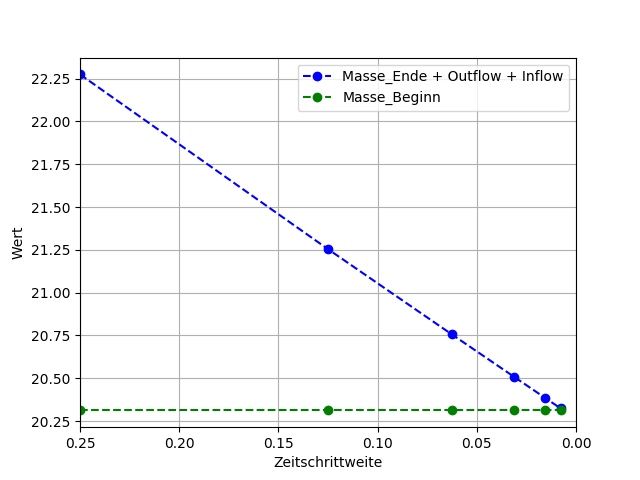
\includegraphics[width=0.8\textwidth]{../Aufgabe21/massoverdt2.png}
\end{figure}


Betrachten wir nun hingegen in Abbildung 5 den zeitlichen Verlauf der Energie, so stellen wir schnell fest, dass diese nicht erhalten wird. Dies deckt sich mit den theoretischen Resultaten der Vorlesung insofern, dass wir für das Finite Volumen Verfahren mit upwind-flux nachgewiesen haben, dass dieser zwar masse- nicht aber energieerhaltend ist. Diese fehlende Energieerhaltung wird im zeitlichen Verlauf sehr gut deutlich. Hier bedarf es also anderen Vorgehensweisen bzw. Verfahren, um auch die Energieerhaltung sicherzustellen.
\newpage
\subsubsection{Problem B (CircleWave)}
Wir setzen für das Problem CircleWave:
\begin{align*}
  \rho_0(x,y) &= 
  \left\{ 
    \begin{array}{r l}
      (\cos(\frac{1}{2 \pi}r)+1)^2,& 
      r = \left| 
      \begin{pmatrix}
        x \\ y \end{pmatrix} 
      - 
      \begin{pmatrix}
        2,5 \\ 2,5 \end{pmatrix} \right| < 2  
      \\
      0 ,& \text{sonst}
    \end{array}      
  \right. 
  \\
  \rho_{in} &= 0
\end{align*}

Im Folgenden betrachten wir für dieses Problem die transportierte Energie bei einem konzentrischen Fluss zum Anfangs- und Endzeitpunkt. Dabei möchten wir eine möglichst gute Energieerhaltung durch die Verfahren erhalten. Wir vergleichen die Qualität der Finite Volumen Methode (deg = 0) mit dem Discontinuous Galerkin Verfahren 2. Ordnung (deg = 2). Zuerst betrachten wir die Lösung der Finite 
Volumen Methode auf Level 6.
\begin{figure}[H]
	\centering
	\captionabove{CircleWave mit Finite Volumen}
    \subfigure[$t = 0$]{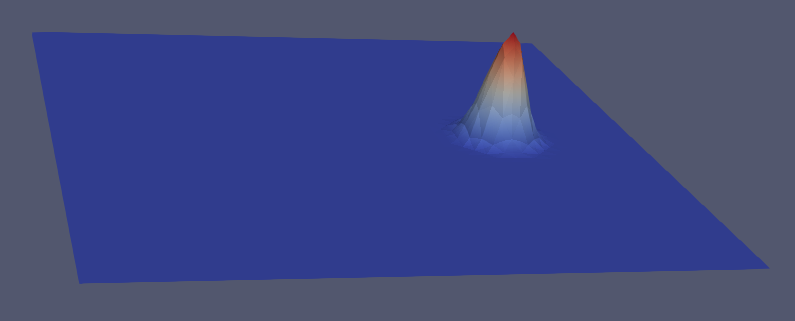
\includegraphics[width=0.47\textwidth]{../CircleWaveDeg0Level6/animation0schnitt.png}}
	\subfigure[$t = 0,125$]{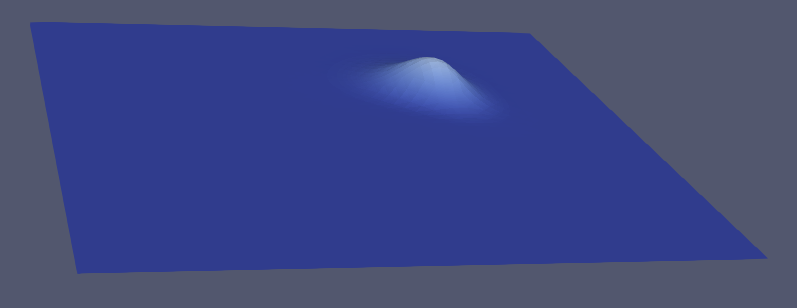
\includegraphics[width=0.49\textwidth]{../CircleWaveDeg0Level6/animation2schnitt.png}}
	\subfigure[$t = 1$]{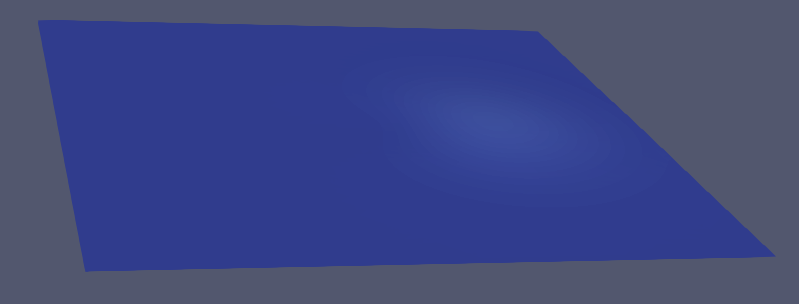
\includegraphics[width=0.49\textwidth]{../CircleWaveDeg0Level6/animation16schnitt.png}}
\end{figure}

Anhand des ersten Bildes können wir die Energie im Ausgangszustand erkennen. Diese nimmt schon zu Beginn rapide ab. Bereits zum Zeitpunkt $t = 0,125$ ist die Energie deutlich geringer und zum Endzeitpunkt ($t=1$) nahezu $0$. Diese
Beobachtung bestätigt sich mithilfe der folgenden Tabelle:

\begin{figure}[H]
	\centering
	\captionabove{deg = 0, Problem = CircleWave, Finite Volumen,
	Energie}
	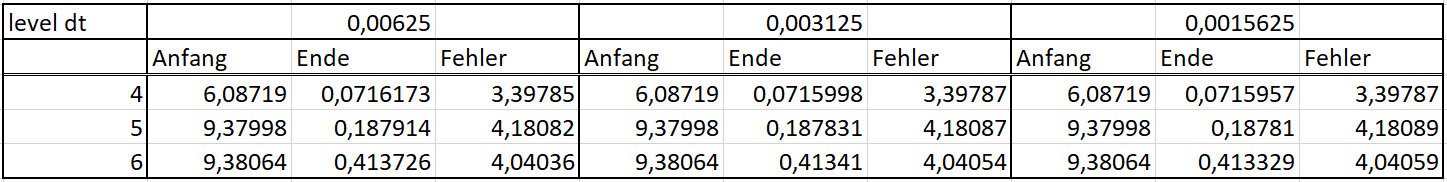
\includegraphics[width=\textwidth]{../Aufgabe21/deg=0CircleWaveEnergieTabelle.png}
\end{figure}

Anhand der Tabelle erkennen wir, dass die Energie zum Endzeitpunkt auf allen Levels nicht mal mehr 10 \% der Anfangsenergie beträgt. Daraus resultiert auch der hohe Fehlerwert ($\approx 4$). 
Betrachten wir nun das Discontinuous Galerkin Verfahren 2. Ordnung (DGV) auf Level 5:

\begin{figure}[H]
	\centering
	\captionabove{CircleWave, Deg = 2, Level 5, dt = 0,00625}
    \subfigure[t = 0]{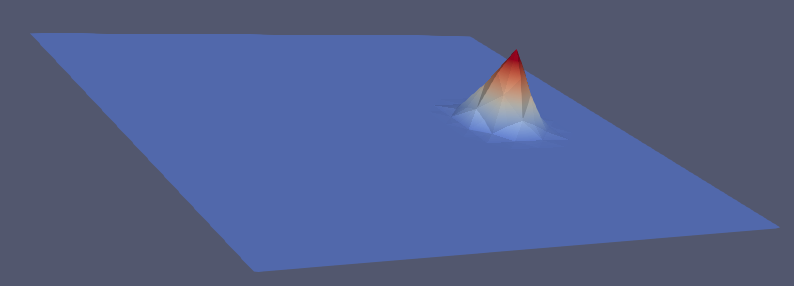
\includegraphics[width=0.48\textwidth]{../CircleWaveDeg2Level5/animation0schnitt.png}}
	\subfigure[t = 0,125]{
\includegraphics[width=0.49\textwidth]{../CircleWaveDeg2Level5/animation2schnitt.png}}
	\subfigure[t = 1]{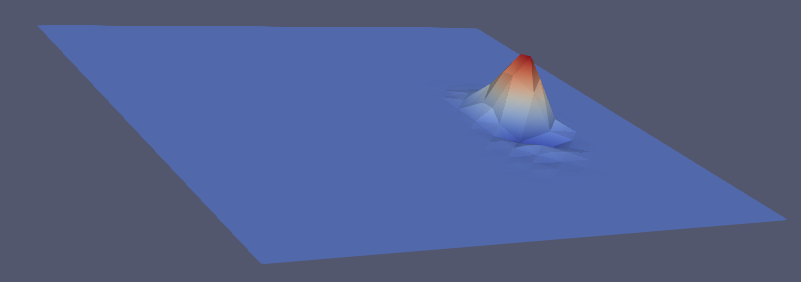
\includegraphics[width=0.49\textwidth]{../CircleWaveDeg2Level5/animation16schnitt.png}}
\end{figure}

Im Vergleich der beiden Bilder zum Startzeitpunkt $t=0$ und Endzeitpunkt $t=1$ erkennen wir, dass das DGV die Energie fast vollständig erhalten hat. Auch hier zeigt ein Blick in die Wertetabelle, dass sich unsere Beobachtung bestätigt.

\begin{figure}[H]
	\centering
	\captionabove{CircleWave mit DGV}
	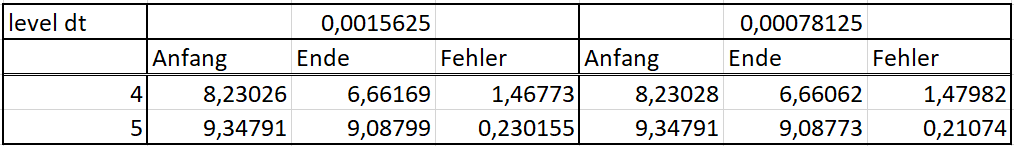
\includegraphics[width=\textwidth]{../Aufgabe21/deg=2CircleWaveEnergieTabelle.png}
\end{figure}

Bereits bei Level 5 erhalten wir sehr gute Ergebnisse.
Die Werte der Energie zum Start- und Endzeitpunkt sind hier nahe beieinander und somit liefert uns das DGV eine fast vollständige Energieerhaltung. Auch die Fehlerwert auf Level 5 ($\approx 0,21$) sind im Vergleich zu den Finite Volumen sehr gering. Zusammenfassend können wir damit festhalten, dass lediglich das DGV für das Problem CircleWave energieerhaltend ist und zufriedenstellende Ergebnisse liefert.



\newpage
\subsection{Aufgabe 24}
In dieser Aufgabe betrachten wir die Versickerung von Öl. Dabei lösen wir wie in Aufgabe 21 Teil B zuerst mit der Finite Volumen Methode und dann mit dem DGV.
\begin{figure}[H]
	\centering
	\captionabove{Finite Volumen}
    \subfigure[t = 0]{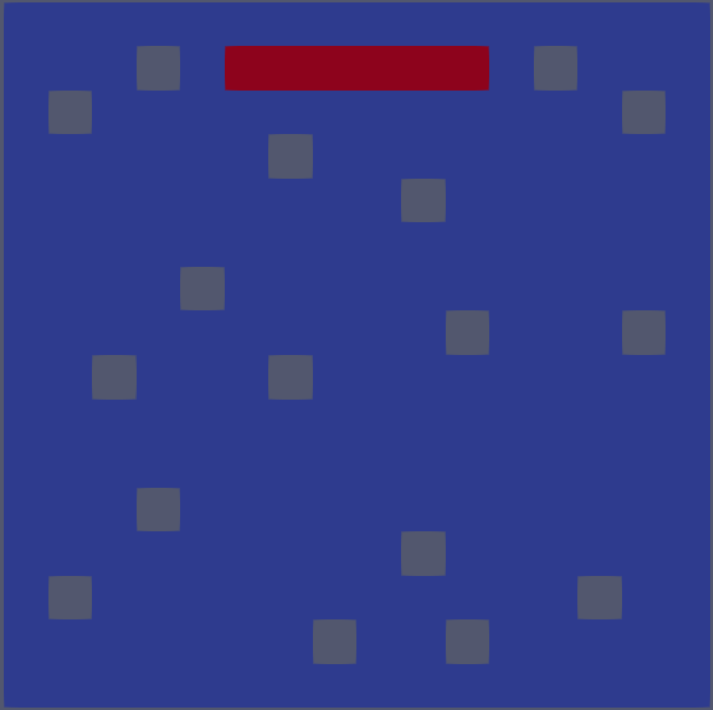
\includegraphics[width=0.49\textwidth]{../Aufgabe24/Level2Deg0/animation1.png}}
	\subfigure[t = 0,15]{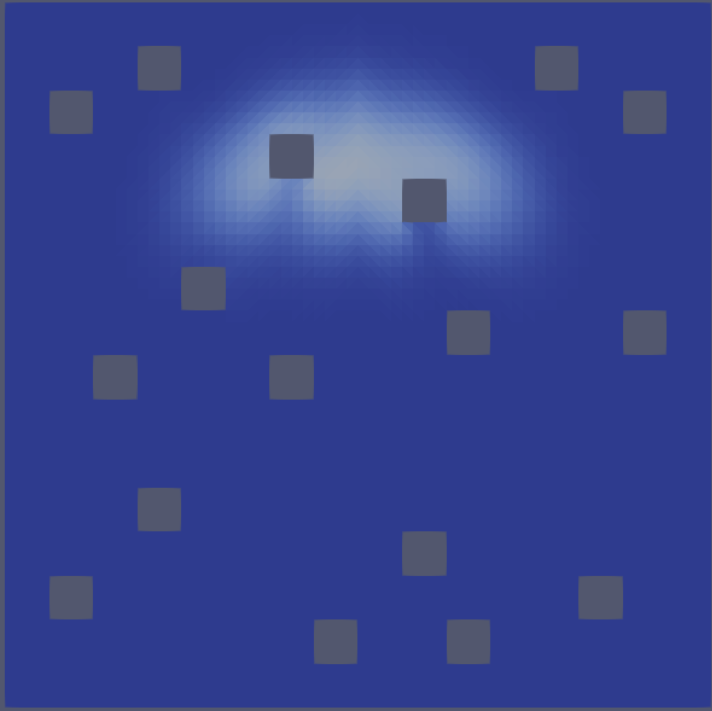
\includegraphics[width=0.49\textwidth]{../Aufgabe24/Level2Deg0/animation2.png}}
	\subfigure[t = 0,85]{
\includegraphics[width=0.49\textwidth]{../Aufgabe24/Level2Deg0/animation3.png}}
\end{figure}
Wie wir anhand der Bilder erkennen können, verschwindet beim Finite Volumen Verfahren wie in Aufgabe 21 schnell ein Großteil der Energie. An den Schaubildern erkennt man das daran, dass die Lösung relativ schnell 'verwischt'. Im Gegensatz dazu sieht man bei dem DGV, dass die Energie nahezu erhalten wird.

\begin{figure}[H]
	\centering
	\captionabove{Discontinuous Galerkin Verfahren 2. Ordnung}
    \subfigure[t = 0]{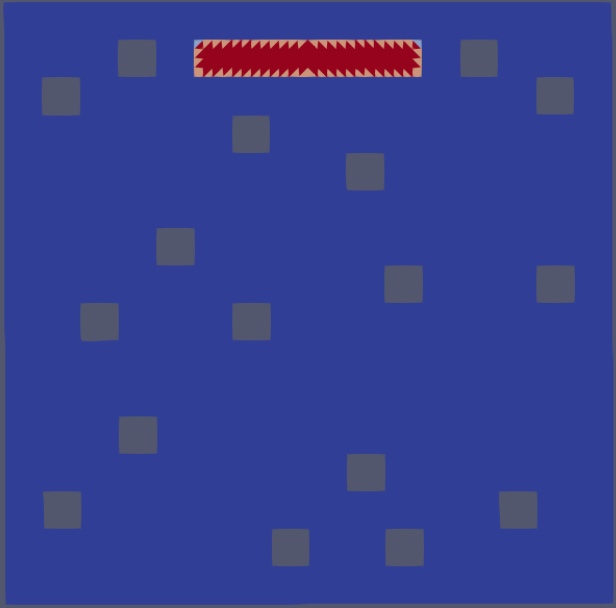
\includegraphics[width=0.49\textwidth]{../Aufgabe24/Level2Deg2/animation1.png}}
	\subfigure[t = 0,15]{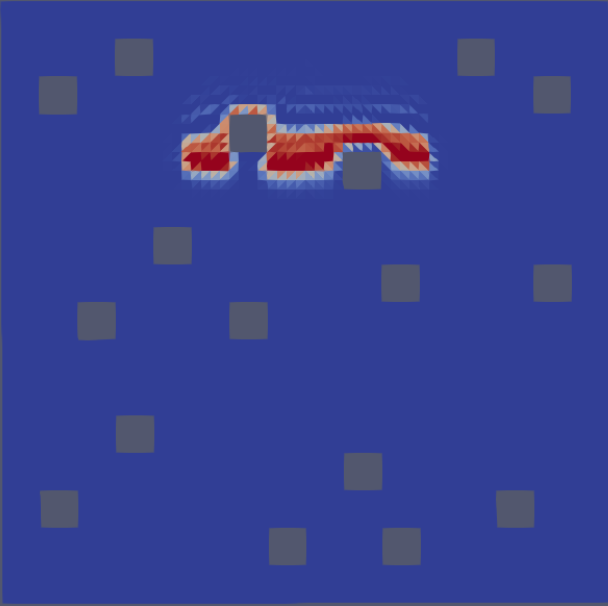
\includegraphics[width=0.49\textwidth]{../Aufgabe24/Level2Deg2/animation2.png}}
	\subfigure[t = 0,7]{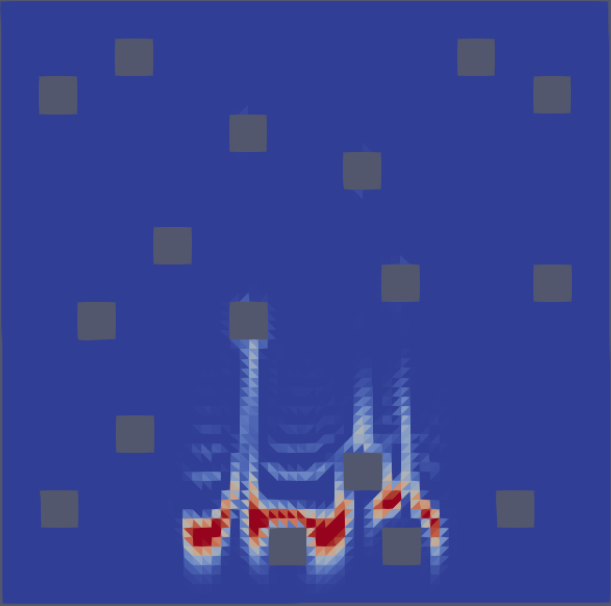
\includegraphics[width=0.49\textwidth]{../Aufgabe24/Level2Deg2/animation3.png}}
\end{figure}

Dafür sieht man aber, dass beim DGV 2. Ordnung die Positivität bzw. Monotonie nicht erhalten bleibt. Dies erkennt man einerseits an den 3-dimensionalen Lösungsplots

\begin{figure}[H]
	\centering
	\captionabove{Lösungsplot}
    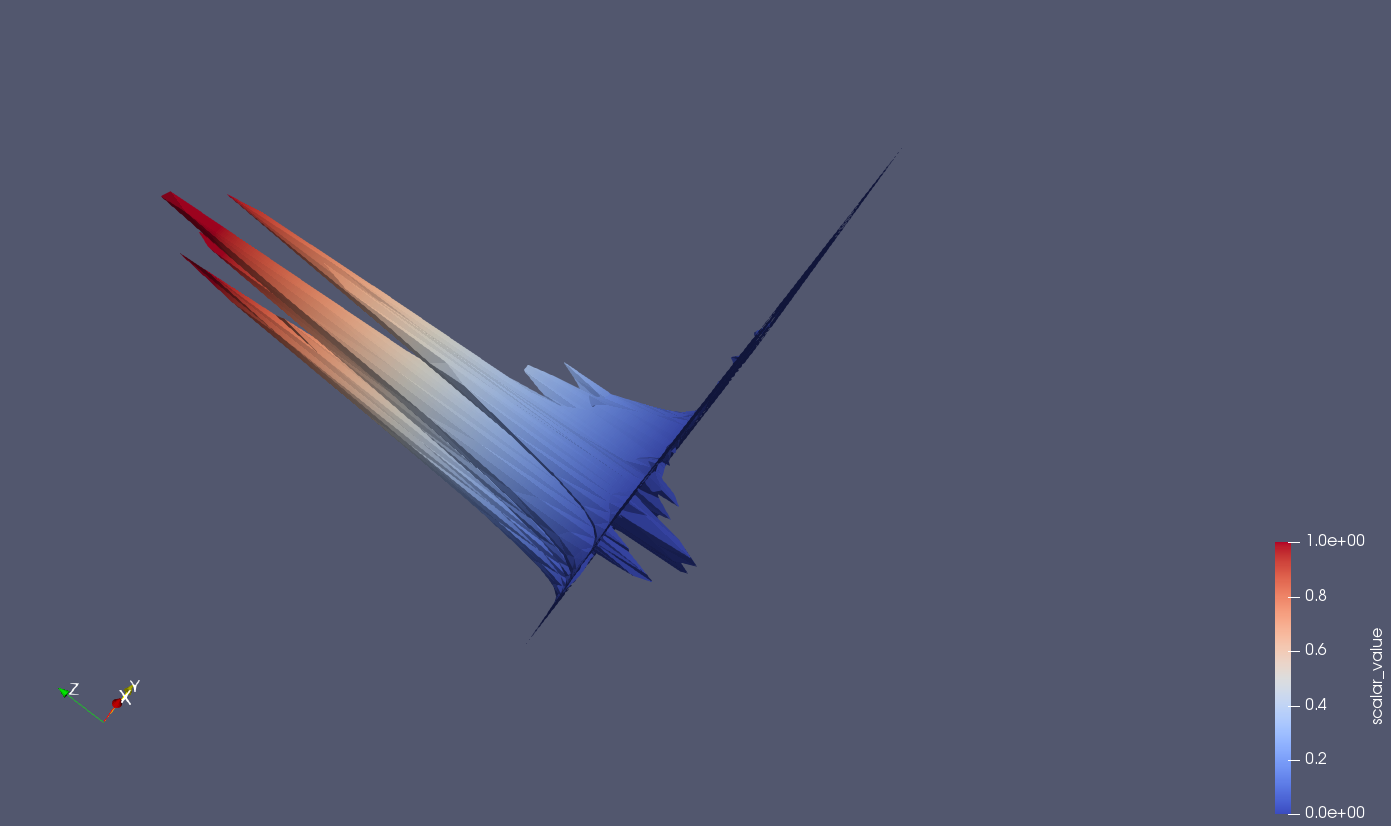
\includegraphics[width=0.99\textwidth]{../Aufgabe24/Level2Deg2/negativ.png}
\end{figure}
andererseits erkennt man das auch an den Ausflussplots:


\begin{figure}[H]
	\centering
	\captionabove{Ausflussplots}

	\subfigure[lvl 2 deg 2]{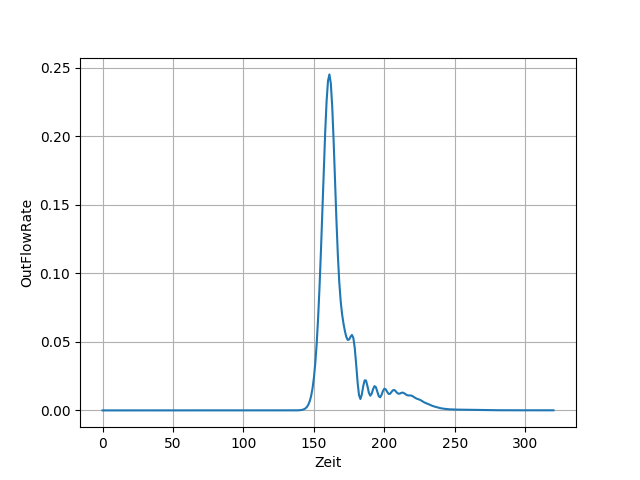
\includegraphics[width=0.49\textwidth]{../Aufgabe24/Level2Deg2.png}}
	\subfigure[lvl 2 deg 0]{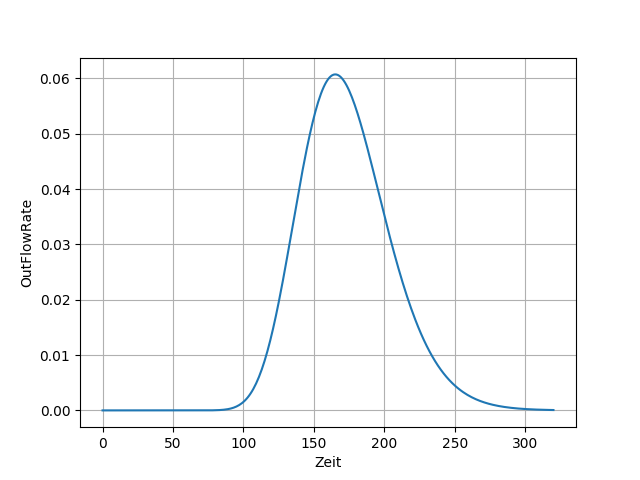
\includegraphics[width=0.49\textwidth]{../Aufgabe24/Level2Deg0.png}}
\end{figure}



